\documentclass{beamer}

\usepackage[utf8]{inputenc}

\usetheme{Warsaw}

\useoutertheme{infolines}
\setbeamertemplate{blocks}[default]
\hypersetup{linkbordercolor={ 0.36 1 0.54 }}
%% \setbeamertemplate{items}[circle]

% \logo{\includegraphics[width=15px,height=15px]{/home/wulczer/flumotion.png}}

\AtBeginSubsection[]
{
  \begin{frame}{Outline}
    \tableofcontents[sectionstyle=show/shaded,subsectionstyle=show/shaded/hide]
  \end{frame}
}

\title{Replacing GEQO}
\subtitle{Join ordering via Simulated Annealing}
\author{Jan Urbanski \\ \texttt{j.urbanski@wulczer.org}}
\institute{University of Warsaw / Flumotion}
\date{\today}

\begin{document}

\frame{\titlepage}

\begin{frame}
  \tableofcontents
\end{frame}

\section{The problem}
\subsection{Determining join order for large queries}

\begin{frame}
  \frametitle{Getting the optimal join order}

  \begin{itemize}
  \item part of of planning a query is determining the order in which relations
    are joined
  \item it is not unusual to have queries that join lots of relations
  \item JOIN and subquery flattening contributes to the number or relations to
    join
  \item automatically generated queries can involve very large joins
  \end{itemize}
\end{frame}

\begin{frame}
  \frametitle{Problems with join ordering}

  \begin{itemize}
  \item finding the optimal join order is an NP-hard problem
  \item considering all possible ways to do a join can exhaust available memory
  \item not all join orders are valid, because of:
    \begin{itemize}
    \item outer joins enforcing a certain join order
    \item IN and EXISTS clauses that get converted to joins
    \end{itemize}
  \item joins with restriction clauses are preferable to Cartesian joins
  \end{itemize}
\end{frame}

\subsection{GEQO, the genetic query optimiser}

\begin{frame}
  \frametitle{Randomisation helps}

  \begin{itemize}
  \item PostgreSQL switches from exhaustive search to a randomised algorithm
    after a certain limit
  \item GEQO starts by joining the relations in any order
  \item and then proceeds to randomly change the join order
  \item genetic algorithm techniques are used to choose the cheapest join order
  \end{itemize}
\end{frame}

\begin{frame}
  \frametitle{Problems with GEQO}

  \begin{itemize}
  \item has lots of dead/experimental code
  \item there is a TODO item to remove it
  \item nobody really cares about it
  \item is an adaptation of an algorithm to solve TSP, not necessarily best
    suited to join ordering
  \item requires some cooperation from the planeer, which violates abstractions
  \end{itemize}
\end{frame}

\section{The solution}

\subsection{Simulated Annealing overview}

\begin{frame}
  \frametitle{Previous work}
  FIXME

  Twopo, the paper by the Greek, suggestions on the mailing list.
\end{frame}

\begin{frame}
  \frametitle{What is Simulated Annealing}

  \begin{columns}
    \begin{column}{7cm}
      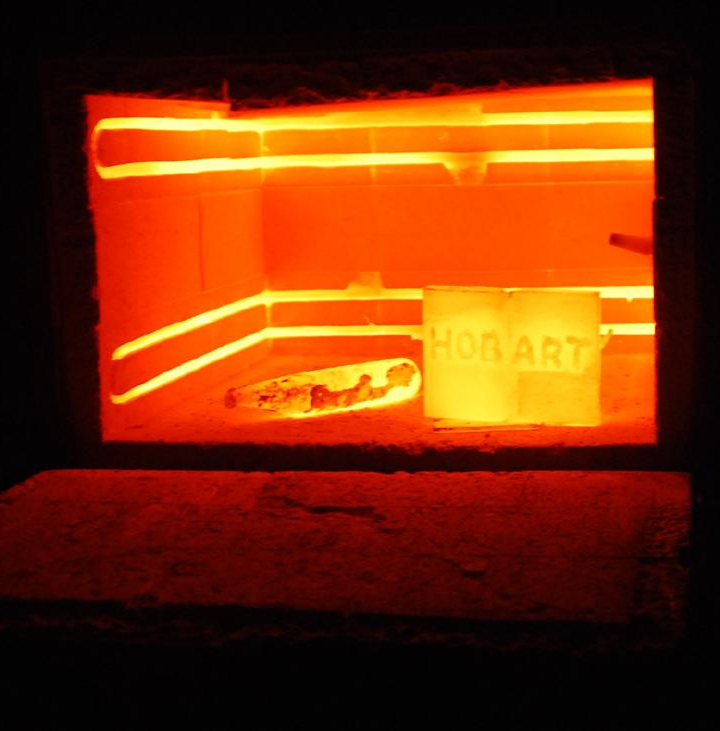
\includegraphics[width=7cm]{furnace.png}
    \end{column}
    \begin{column}{5cm}
      Annealing (...) is a process that produces conditions by heating to above
      the re-crystallization temperature and maintaining a suitable
      temperature, and then cooling.\\
      \hfill\textit{-- Wikipedia}
    \end{column}
  \end{columns}
\end{frame}

\begin{frame}
  \frametitle{The SA Algorithm cont.}

  \begin{itemize}
  \item the system starts with an initial temperature and a random state
  \item uphill moves are accepted with probability that depends on the current
    temperature
    \begin{block}{probability of accepting an uphill move}
      \begin{equation*}
        p = e^{\frac{cost_{prev} - cost_{new}}{temperature}}
      \end{equation*}
    \end{block}
  \item moves are made until equilibrium is reached
  \item temperature is gradually lowered
  \item once the system is frozen, the algorithm ends
  \end{itemize}

\end{frame}

\begin{frame}<-6>[fragile,label=sa-algorithm]
  \frametitle{The SA algorithm}

\begin{block}{Simulated Annealing}
\begin{semiverbatim}
\uncover<2->{state = \alert<7->{random\_state()}}
\uncover<6->{do \{}
\uncover<4->{    do \{}
\uncover<3->{      new\_state = \alert<8->{random\_move()}}
\uncover<3->{      if (\alert<9->{acceptable(}new\_state\alert<9->{)})}
\uncover<3->{        state = new\_state}
\uncover<4->{    \}}
\uncover<4->{    while (!\alert<10->{equilibrium()})}
\uncover<5->{    \alert<11->{reduce\_temperature()}}
\uncover<6->{\}}
\uncover<6->{while (!\alert<12->{frozen()})}
\uncover<6->{return state}
\end{semiverbatim}
\end{block}

\end{frame}

\begin{frame}<1>[label=sa-problems]
  \frametitle<1>{The SA Algorithm cont.}
  %% \frametitle<2->{SA Algorithm problems}

Implementing Simulated Annealing means solving the following problems:

  \begin{itemize}
  \item \structure<3->{finding an initial state}
  \item \alert<4->{generating subsequent states}
  \item \structure<3->{defining an acceptance function}
  \item \structure<3->{determining the equilibrium condition}
  \item \structure<3->{suitably lowering the temperature}
  \item \structure<3->{determining the freeze conditions}
  \end{itemize}

  \begin{center}
    \only<3->{Some are \structure{easy}}\only<4->{, some are \alert{hard}}
  \end{center}
\end{frame}

\againframe<6->{sa-algorithm}

\begin{frame}
  \frametitle{A visual example}
  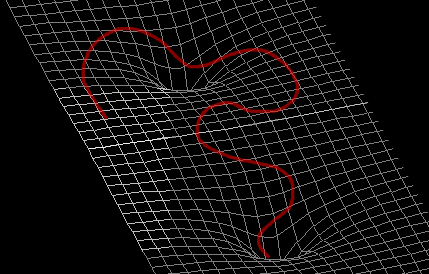
\includegraphics[width=\textwidth]{curve.png}
\end{frame}

\subsection{PostgreSQL specifics}

\begin{frame}
  \frametitle{Differences from the original algorithm}

  \begin{itemize}
  \item PostgreSQL always considers all possible paths for a relation
  \item \texttt{make\_join\_rel} is symmetrical
  \item you can have join order constraints (duh)
  \item the planner is keeping a list of all relations...
  \item ... and sometimes turns it into a hash
  \end{itemize}
\end{frame}

\begin{frame}
  \frametitle{Join order representation}

  \begin{itemize}
  \item SAIO represents joins as \alert{query trees}
  \item chosen to mimic the original algorithm more closely
  \item each state is a query tree
  \item leaves are basic relations
  \item internal nodes are joinrels
  \item the joinrel in the root of the tree is the current result
  \end{itemize}
\end{frame}

\begin{frame}<1>[label=qt-zoom]
  \frametitle<1>{Query trees}
  \framezoom<1><2>[border](1.2cm,0cm)(5.8cm,4.4cm)

  \begin{columns}
    \begin{column}{7cm}
      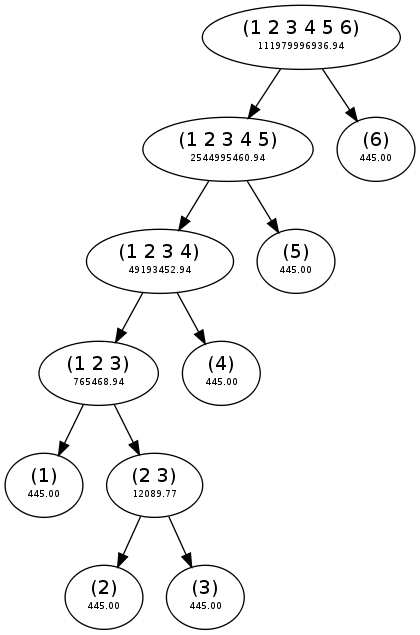
\includegraphics[width=7cm,height=8cm]{qt-example.png}
    \end{column}
    \begin{column}{5cm}
      Example query tree for a six relation join.
    \end{column}
  \end{columns}

\end{frame}

\begin{frame}
  \frametitle{Query trees cont.}

  Some useful query tree properties:

  \begin{itemize}[<+->]
  \item symmetrical (no difference between left and right child)
  \item fully determined by the tree structure and relations in leaves
  \item each node has a cost
  \end{itemize}

  \begin{center}
    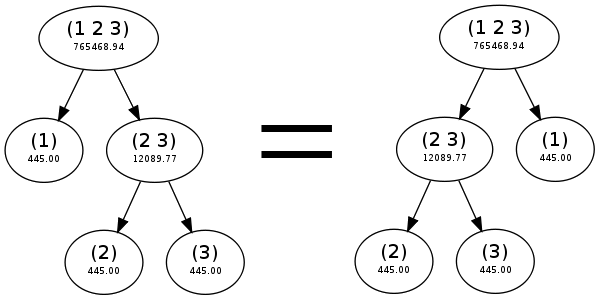
\includegraphics[width=8cm]{qt-symmetrical-1.png}<1>
    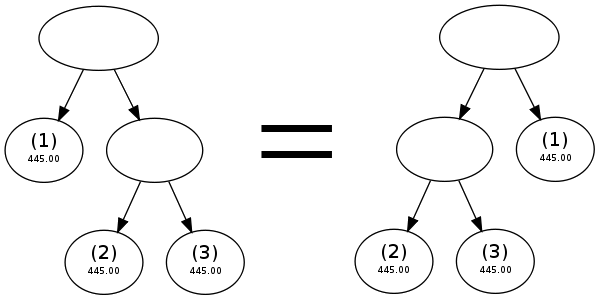
\includegraphics[width=8cm]{qt-symmetrical-2.png}<2>
    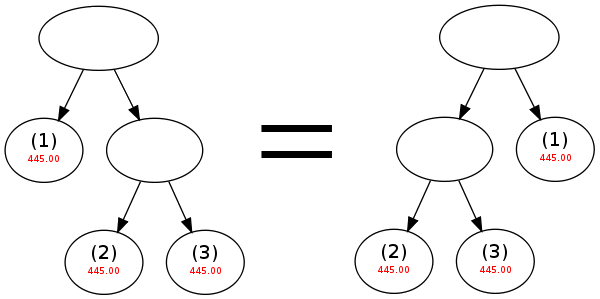
\includegraphics[width=8cm]{qt-symmetrical-3.png}<3>
  \end{center}

\end{frame}

\subsection{Query tree transformations}

\againframe<2->{sa-problems}

\begin{frame}
  \frametitle{The easy problems - initial state}

  \begin{block}{Finding an initial state}
    Make base relations into one-node trees, keep merging them on joins with
    restriction clases, forcefully merge the remaining ones using Cartesian
    joins. Results in a query tree that is as left-deep as possible.
    \\
    \hfill
    \\
    This is exactly what GEQO does.
  \end{block}
\end{frame}

\begin{frame}
  \frametitle{The easy problems - temperature}

  \begin{block}{The acceptance function}
    A uphill move is accepted with the probability that depends on the current temperature.
    $$P(accepted) = e^{\frac{cost_{prev} - cost_{new}}{temperature}}$$
  \end{block}

  \begin{block}{Lowering the temperature}
    The initial temperature depends on the number of initial relations and
    drops geometrically.
    $$initial\_temperature = I * initial\_rels$$
    $$new\_temperature = temperature * K$$ where $$0 < K < 1$$
  \end{block}
\end{frame}

\begin{frame}
  \frametitle{The easy problems - equilibrium and freezing}

  \begin{block}{Equilibrium condition}
    Equilibrium is reached after a fixed number of moves that depend on the
    number of initial relations.
    $$moves\_to\_equilibrium = N * initial\_rels$$
  \end{block}

  \begin{block}{Freezing condition}
    The system freezes if temperature falls below 1 and a fixed number of
    consecutive moves has failed.
  \end{block}
\end{frame}

\begin{frame}
  \frametitle{Move types}

  The difficult part seems to be generating subsequent states.

  \begin{itemize}
  \item a number of move generating approaches can be taken
  \item the most costly operations is creating a joinrel, especially computing
    paths
  \item need to free memory between steps, otherwise risk overrunning
  \item need to deal with planner scribbling on its structures when creating
    joinrels
  \item how to efficiently sample the solution space?
  \end{itemize}
\end{frame}

\begin{frame}
  \frametitle{SAIO \texttt{move}}

  \begin{itemize}
  \item randomly choose two nodes from the query tree
  \item swap the subtrees around
  \item recalculate the whole query tree
  \item if it cannot be done, the move fails
  \item check if the cost of the new tree is acceptable
  \item if not, the move fails
  \end{itemize}
\end{frame}

\begin{frame}
  \frametitle{SAIO \texttt{move} example}

  \onslide<1->{Take a tree,}
  \onslide<2->{choose two nodes,}
  \onslide<3->{swap them around}

  \begin{columns}[b]
    \begin{column}{6.2cm}
      \includegraphics<1>[width=6.2cm,height=6.9cm]{saio-move-1.png}
      \includegraphics<2->[width=6.2cm,height=6.9cm]{saio-move-2.png}
    \end{column}
    \begin{column}{6.2cm}
      \includegraphics<3->[width=6.2cm]{saio-move-3.png}
    \end{column}
  \end{columns}
\end{frame}

\begin{frame}
  \frametitle{SAIO \texttt{move} problems}

  \begin{itemize}
  \item choosing a node narrows down the possible choices for the second node
    \begin{itemize}
    \item can't choose descendant node (how would that work?)
    \item can't choose ancestor node (for the same reason)
    \item can't choose sibling node (because of symmetry)
    \end{itemize}
  \item the changes to the tree are big, the algorithm takes ``large steps''
  \item if the resulting query tree is invalid, lots of work is thrown away
  \item any join failure results in the whole move failing, so it doesn't
    explore the solution space very deeply
  \end{itemize}
\end{frame}

\begin{frame}
  \frametitle{SAIO \texttt{pivot}}

  \begin{itemize}
  \item change \texttt{(A join B) join C} into \texttt{A join (B join C)}
  \item in practise, choose a node at random
  \item swap the subtrees of one of its children and the sibling's
  \item continue trying such pivots until all nodes have been tried
  \end{itemize}
\end{frame}

\begin{frame}
  \frametitle{SAIO \texttt{pivot} example}

  \onslide<1->{Take a tree,}
  \onslide<2->{choose a node,}
  \onslide<3->{pivot,}
  \onslide<4->{choose another,}
  \onslide<5->{pivot ...}

  \begin{columns}[b]
    \begin{column}{6.2cm}
      \includegraphics<1>[width=6.2cm,height=6.9cm]{saio-pivot-1.png}
      \includegraphics<2-3>[width=6.2cm,height=6.9cm]{saio-pivot-2.png}
      \includegraphics<4->[width=6.2cm,height=6.9cm]{saio-pivot-4.png}
    \end{column}
    \begin{column}{6.2cm}
      \includegraphics<3>[width=6.2cm]{saio-pivot-3.png}
      \includegraphics<4>[width=6.2cm]{saio-pivot-5.png}
      \includegraphics<5->[width=6.2cm]{saio-pivot-6.png}
    \end{column}
  \end{columns}
\end{frame}

\begin{frame}
  \frametitle{SAIO \texttt{pivot} problems}

  \begin{itemize}
  \item each move explores a lot of possibilities, but requires lots of
    computation
  \item does not introduce big changes, which sometimes are needed to break
    pessimal joins
    \begin{itemize}
    \item actually, it's not obvious that the solution space is smooth wrt
      costs
    \item small changes in the structure may result it gigantic changes in
      costs
    \item might want to augment the cost assesment function (number of
      non-cross joins?)
    \end{itemize}
  \item the same join might be recalculated many times in each step
  \end{itemize}
\end{frame}

\begin{frame}
  \frametitle{SAIO \texttt{recalc}}

  \begin{itemize}
  \item essentialy the same as \texttt{move}
  \item recalculate the joins from the chosen nodes up to the common ancestor
  \item if it succeeded, recalculate the nodes from the common ancestor up to
    the root node
  \item avoids pointless recalculations when joins fail
  \end{itemize}
\end{frame}

\begin{frame}
  \frametitle{SAIO \texttt{recalc} example}

  %% \includegraphics<1->[width=\textwidth]{saio-recalc-1.png}
  %% \includegraphics<2->[width=\textwidth]{saio-recalc-2.png}
  %% \includegraphics<3->[width=\textwidth]{saio-recalc-3.png}
  %% \includegraphics<4->[width=\textwidth]{saio-recalc-4.png}
\end{frame}

\begin{frame}
  \frametitle{SAIO \texttt{recalc} problems}

  \begin{itemize}
  \item does really nasty hacks
  \item does not speed things up as much as it should
  \item probably need a different approach
  \end{itemize}
\end{frame}

\section{The results}
\subsection{Comparison with GEQO}

\section{The future}
\subsection{Development focuses}

\begin{frame}
  \frametitle{What the future brings}

  \begin{itemize}
  \item MSc thesis :o)
  \item smarter tree transformation methods
  \item less useless computation
  \item perhaps some support from the core infrastructure
  \item faster and higher quality results than GEQO
  \item \texttt{git://wulczer.org/saio.git}
  \end{itemize}
\end{frame}

\begin{frame}
  \frametitle{Acknowledgements}

  \begin{itemize}
  \item Adriano Lange, the author of the TWOPO implementation
  \item Andres Freund, for providing the craziest test query ever
  \item Robert Haas, for providing a slightly less crazy test query
  \item dr Krzysztof Stencel, for help and guidance
  \item Flumotion Services, for letting me mess with the PG planner instead of
    doing work
  \end{itemize}
\end{frame}

\begin{frame}
  \frametitle{Further reading}

  \begin{thebibliography}{Steinbrunn 1997}

  \bibitem[Ioannidis 1987]{ioannidis}
    Yannis~E. Ioannidis and Eugene Wong.
    \newblock Query optimization by simulated annealing.
    \newblock {\em SIGMOD Rec.}, 16(3):9--22, 1987.

  \bibitem[Steinbrunn 1997]{steinbrunn}
    Michael Steinbrunn, Guido Moerkotte, and Alfons Kemper.
    \newblock Heuristic and randomized optimization for the join ordering problem.
    \newblock {\em The VLDB Journal}, 6(3):191--208, 1997.

  \end{thebibliography}
\end{frame}

\section{The end}
\subsection*{Questions}

\begin{frame}
\begin{beamercolorbox}[center]{note}
  \Huge Questions?
\end{beamercolorbox}
\end{frame}

\appendix

\againframe<2>[plain]{qt-zoom}

\end{document}
